% Created by tikzDevice version 0.12 on 2019-04-02 22:26:33
% !TEX encoding = UTF-8 Unicode
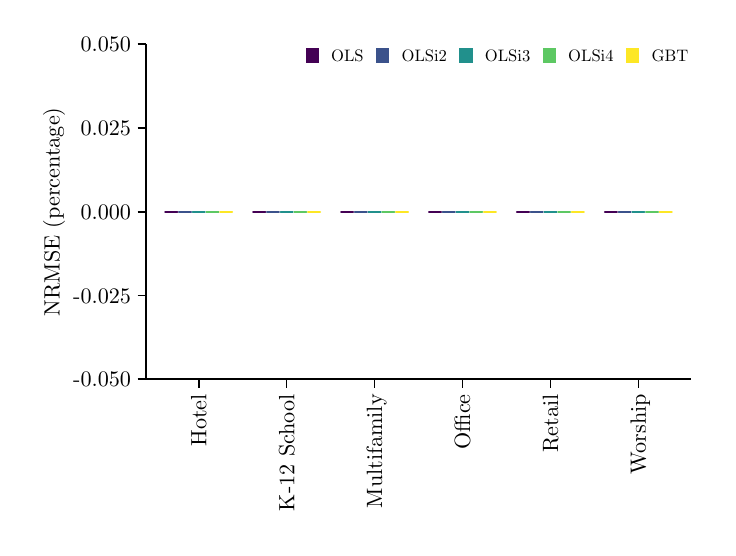
\begin{tikzpicture}[x=1pt,y=1pt]
\definecolor{fillColor}{RGB}{255,255,255}
\path[use as bounding box,fill=fillColor,fill opacity=0.00] (0,0) rectangle (245.72,180.67);
\begin{scope}
\path[clip] (  0.00,  0.00) rectangle (245.72,180.67);
\definecolor{drawColor}{RGB}{255,255,255}
\definecolor{fillColor}{RGB}{255,255,255}

\path[draw=drawColor,line width= 0.6pt,line join=round,line cap=round,fill=fillColor] (  0.00,  0.00) rectangle (245.72,180.68);
\end{scope}
\begin{scope}
\path[clip] ( 42.74, 53.61) rectangle (239.72,174.67);
\definecolor{fillColor}{RGB}{255,255,255}

\path[fill=fillColor] ( 42.74, 53.61) rectangle (239.72,174.67);
\definecolor{drawColor}{RGB}{253,231,37}
\definecolor{fillColor}{RGB}{253,231,37}

\path[draw=drawColor,line width= 0.6pt,line join=round,fill=fillColor] ( 69.49,114.14) rectangle ( 73.94,114.14);
\definecolor{drawColor}{RGB}{93,200,99}
\definecolor{fillColor}{RGB}{93,200,99}

\path[draw=drawColor,line width= 0.6pt,line join=round,fill=fillColor] ( 64.53,114.14) rectangle ( 68.98,114.14);
\definecolor{drawColor}{RGB}{33,144,140}
\definecolor{fillColor}{RGB}{33,144,140}

\path[draw=drawColor,line width= 0.6pt,line join=round,fill=fillColor] ( 59.58,114.14) rectangle ( 64.02,114.14);
\definecolor{drawColor}{RGB}{59,82,139}
\definecolor{fillColor}{RGB}{59,82,139}

\path[draw=drawColor,line width= 0.6pt,line join=round,fill=fillColor] ( 54.62,114.14) rectangle ( 59.07,114.14);
\definecolor{drawColor}{RGB}{68,1,84}
\definecolor{fillColor}{RGB}{68,1,84}

\path[draw=drawColor,line width= 0.6pt,line join=round,fill=fillColor] ( 49.66,114.14) rectangle ( 54.11,114.14);
\definecolor{drawColor}{RGB}{253,231,37}
\definecolor{fillColor}{RGB}{253,231,37}

\path[draw=drawColor,line width= 0.6pt,line join=round,fill=fillColor] (101.26,114.14) rectangle (105.71,114.14);
\definecolor{drawColor}{RGB}{93,200,99}
\definecolor{fillColor}{RGB}{93,200,99}

\path[draw=drawColor,line width= 0.6pt,line join=round,fill=fillColor] ( 96.30,114.14) rectangle (100.75,114.14);
\definecolor{drawColor}{RGB}{33,144,140}
\definecolor{fillColor}{RGB}{33,144,140}

\path[draw=drawColor,line width= 0.6pt,line join=round,fill=fillColor] ( 91.35,114.14) rectangle ( 95.80,114.14);
\definecolor{drawColor}{RGB}{59,82,139}
\definecolor{fillColor}{RGB}{59,82,139}

\path[draw=drawColor,line width= 0.6pt,line join=round,fill=fillColor] ( 86.39,114.14) rectangle ( 90.84,114.14);
\definecolor{drawColor}{RGB}{68,1,84}
\definecolor{fillColor}{RGB}{68,1,84}

\path[draw=drawColor,line width= 0.6pt,line join=round,fill=fillColor] ( 81.43,114.14) rectangle ( 85.88,114.14);
\definecolor{drawColor}{RGB}{253,231,37}
\definecolor{fillColor}{RGB}{253,231,37}

\path[draw=drawColor,line width= 0.6pt,line join=round,fill=fillColor] (133.03,114.14) rectangle (137.48,114.14);
\definecolor{drawColor}{RGB}{93,200,99}
\definecolor{fillColor}{RGB}{93,200,99}

\path[draw=drawColor,line width= 0.6pt,line join=round,fill=fillColor] (128.07,114.14) rectangle (132.52,114.14);
\definecolor{drawColor}{RGB}{33,144,140}
\definecolor{fillColor}{RGB}{33,144,140}

\path[draw=drawColor,line width= 0.6pt,line join=round,fill=fillColor] (123.12,114.14) rectangle (127.57,114.14);
\definecolor{drawColor}{RGB}{59,82,139}
\definecolor{fillColor}{RGB}{59,82,139}

\path[draw=drawColor,line width= 0.6pt,line join=round,fill=fillColor] (118.16,114.14) rectangle (122.61,114.14);
\definecolor{drawColor}{RGB}{68,1,84}
\definecolor{fillColor}{RGB}{68,1,84}

\path[draw=drawColor,line width= 0.6pt,line join=round,fill=fillColor] (113.21,114.14) rectangle (117.65,114.14);
\definecolor{drawColor}{RGB}{253,231,37}
\definecolor{fillColor}{RGB}{253,231,37}

\path[draw=drawColor,line width= 0.6pt,line join=round,fill=fillColor] (164.80,114.14) rectangle (169.25,114.14);
\definecolor{drawColor}{RGB}{93,200,99}
\definecolor{fillColor}{RGB}{93,200,99}

\path[draw=drawColor,line width= 0.6pt,line join=round,fill=fillColor] (159.85,114.14) rectangle (164.29,114.14);
\definecolor{drawColor}{RGB}{33,144,140}
\definecolor{fillColor}{RGB}{33,144,140}

\path[draw=drawColor,line width= 0.6pt,line join=round,fill=fillColor] (154.89,114.14) rectangle (159.34,114.14);
\definecolor{drawColor}{RGB}{59,82,139}
\definecolor{fillColor}{RGB}{59,82,139}

\path[draw=drawColor,line width= 0.6pt,line join=round,fill=fillColor] (149.93,114.14) rectangle (154.38,114.14);
\definecolor{drawColor}{RGB}{68,1,84}
\definecolor{fillColor}{RGB}{68,1,84}

\path[draw=drawColor,line width= 0.6pt,line join=round,fill=fillColor] (144.98,114.14) rectangle (149.42,114.14);
\definecolor{drawColor}{RGB}{253,231,37}
\definecolor{fillColor}{RGB}{253,231,37}

\path[draw=drawColor,line width= 0.6pt,line join=round,fill=fillColor] (196.57,114.14) rectangle (201.02,114.14);
\definecolor{drawColor}{RGB}{93,200,99}
\definecolor{fillColor}{RGB}{93,200,99}

\path[draw=drawColor,line width= 0.6pt,line join=round,fill=fillColor] (191.62,114.14) rectangle (196.06,114.14);
\definecolor{drawColor}{RGB}{33,144,140}
\definecolor{fillColor}{RGB}{33,144,140}

\path[draw=drawColor,line width= 0.6pt,line join=round,fill=fillColor] (186.66,114.14) rectangle (191.11,114.14);
\definecolor{drawColor}{RGB}{59,82,139}
\definecolor{fillColor}{RGB}{59,82,139}

\path[draw=drawColor,line width= 0.6pt,line join=round,fill=fillColor] (181.70,114.14) rectangle (186.15,114.14);
\definecolor{drawColor}{RGB}{68,1,84}
\definecolor{fillColor}{RGB}{68,1,84}

\path[draw=drawColor,line width= 0.6pt,line join=round,fill=fillColor] (176.75,114.14) rectangle (181.20,114.14);
\definecolor{drawColor}{RGB}{253,231,37}
\definecolor{fillColor}{RGB}{253,231,37}

\path[draw=drawColor,line width= 0.6pt,line join=round,fill=fillColor] (228.34,114.14) rectangle (232.79,114.14);
\definecolor{drawColor}{RGB}{93,200,99}
\definecolor{fillColor}{RGB}{93,200,99}

\path[draw=drawColor,line width= 0.6pt,line join=round,fill=fillColor] (223.39,114.14) rectangle (227.84,114.14);
\definecolor{drawColor}{RGB}{33,144,140}
\definecolor{fillColor}{RGB}{33,144,140}

\path[draw=drawColor,line width= 0.6pt,line join=round,fill=fillColor] (218.43,114.14) rectangle (222.88,114.14);
\definecolor{drawColor}{RGB}{59,82,139}
\definecolor{fillColor}{RGB}{59,82,139}

\path[draw=drawColor,line width= 0.6pt,line join=round,fill=fillColor] (213.48,114.14) rectangle (217.92,114.14);
\definecolor{drawColor}{RGB}{68,1,84}
\definecolor{fillColor}{RGB}{68,1,84}

\path[draw=drawColor,line width= 0.6pt,line join=round,fill=fillColor] (208.52,114.14) rectangle (212.97,114.14);
\end{scope}
\begin{scope}
\path[clip] (  0.00,  0.00) rectangle (245.72,180.67);
\definecolor{drawColor}{RGB}{0,0,0}

\path[draw=drawColor,line width= 0.6pt,line join=round] ( 42.74, 53.61) --
	( 42.74,174.67);
\end{scope}
\begin{scope}
\path[clip] (  0.00,  0.00) rectangle (245.72,180.67);
\definecolor{drawColor}{RGB}{0,0,0}

\node[text=drawColor,anchor=base east,inner sep=0pt, outer sep=0pt, scale=  0.80] at ( 37.34, 50.86) {-0.050};

\node[text=drawColor,anchor=base east,inner sep=0pt, outer sep=0pt, scale=  0.80] at ( 37.34, 81.12) {-0.025};

\node[text=drawColor,anchor=base east,inner sep=0pt, outer sep=0pt, scale=  0.80] at ( 37.34,111.39) {0.000};

\node[text=drawColor,anchor=base east,inner sep=0pt, outer sep=0pt, scale=  0.80] at ( 37.34,141.65) {0.025};

\node[text=drawColor,anchor=base east,inner sep=0pt, outer sep=0pt, scale=  0.80] at ( 37.34,171.92) {0.050};
\end{scope}
\begin{scope}
\path[clip] (  0.00,  0.00) rectangle (245.72,180.67);
\definecolor{drawColor}{RGB}{0,0,0}

\path[draw=drawColor,line width= 0.6pt,line join=round] ( 39.74, 53.61) --
	( 42.74, 53.61);

\path[draw=drawColor,line width= 0.6pt,line join=round] ( 39.74, 83.88) --
	( 42.74, 83.88);

\path[draw=drawColor,line width= 0.6pt,line join=round] ( 39.74,114.14) --
	( 42.74,114.14);

\path[draw=drawColor,line width= 0.6pt,line join=round] ( 39.74,144.41) --
	( 42.74,144.41);

\path[draw=drawColor,line width= 0.6pt,line join=round] ( 39.74,174.67) --
	( 42.74,174.67);
\end{scope}
\begin{scope}
\path[clip] (  0.00,  0.00) rectangle (245.72,180.67);
\definecolor{drawColor}{RGB}{0,0,0}

\path[draw=drawColor,line width= 0.6pt,line join=round] ( 42.74, 53.61) --
	(239.72, 53.61);
\end{scope}
\begin{scope}
\path[clip] (  0.00,  0.00) rectangle (245.72,180.67);
\definecolor{drawColor}{RGB}{0,0,0}

\path[draw=drawColor,line width= 0.6pt,line join=round] ( 61.80, 50.61) --
	( 61.80, 53.61);

\path[draw=drawColor,line width= 0.6pt,line join=round] ( 93.57, 50.61) --
	( 93.57, 53.61);

\path[draw=drawColor,line width= 0.6pt,line join=round] (125.34, 50.61) --
	(125.34, 53.61);

\path[draw=drawColor,line width= 0.6pt,line join=round] (157.11, 50.61) --
	(157.11, 53.61);

\path[draw=drawColor,line width= 0.6pt,line join=round] (188.88, 50.61) --
	(188.88, 53.61);

\path[draw=drawColor,line width= 0.6pt,line join=round] (220.66, 50.61) --
	(220.66, 53.61);
\end{scope}
\begin{scope}
\path[clip] (  0.00,  0.00) rectangle (245.72,180.67);
\definecolor{drawColor}{RGB}{0,0,0}

\node[text=drawColor,rotate= 90.00,anchor=base east,inner sep=0pt, outer sep=0pt, scale=  0.80] at ( 64.56, 48.21) {Hotel};

\node[text=drawColor,rotate= 90.00,anchor=base east,inner sep=0pt, outer sep=0pt, scale=  0.80] at ( 96.33, 48.21) {K-12 School};

\node[text=drawColor,rotate= 90.00,anchor=base east,inner sep=0pt, outer sep=0pt, scale=  0.80] at (128.10, 48.21) {Multifamily};

\node[text=drawColor,rotate= 90.00,anchor=base east,inner sep=0pt, outer sep=0pt, scale=  0.80] at (159.87, 48.21) {Office};

\node[text=drawColor,rotate= 90.00,anchor=base east,inner sep=0pt, outer sep=0pt, scale=  0.80] at (191.64, 48.21) {Retail};

\node[text=drawColor,rotate= 90.00,anchor=base east,inner sep=0pt, outer sep=0pt, scale=  0.80] at (223.41, 48.21) {Worship};
\end{scope}
\begin{scope}
\path[clip] (  0.00,  0.00) rectangle (245.72,180.67);
\definecolor{drawColor}{RGB}{0,0,0}

\node[text=drawColor,rotate= 90.00,anchor=base,inner sep=0pt, outer sep=0pt, scale=  0.80] at ( 11.51,114.14) {NRMSE (percentage)};
\end{scope}
\begin{scope}
\path[clip] (  0.00,  0.00) rectangle (245.72,180.67);
\definecolor{fillColor}{RGB}{255,255,255}

\path[fill=fillColor] ( 96.99,165.22) rectangle (239.72,174.67);
\end{scope}
\begin{scope}
\path[clip] (  0.00,  0.00) rectangle (245.72,180.67);
\definecolor{drawColor}{RGB}{68,1,84}
\definecolor{fillColor}{RGB}{68,1,84}

\path[draw=drawColor,line width= 0.6pt,line cap=round,fill=fillColor] (100.70,168.31) rectangle (104.97,172.96);
\end{scope}
\begin{scope}
\path[clip] (  0.00,  0.00) rectangle (245.72,180.67);
\definecolor{drawColor}{RGB}{59,82,139}
\definecolor{fillColor}{RGB}{59,82,139}

\path[draw=drawColor,line width= 0.6pt,line cap=round,fill=fillColor] (126.14,168.31) rectangle (130.41,172.96);
\end{scope}
\begin{scope}
\path[clip] (  0.00,  0.00) rectangle (245.72,180.67);
\definecolor{drawColor}{RGB}{33,144,140}
\definecolor{fillColor}{RGB}{33,144,140}

\path[draw=drawColor,line width= 0.6pt,line cap=round,fill=fillColor] (156.24,168.31) rectangle (160.51,172.96);
\end{scope}
\begin{scope}
\path[clip] (  0.00,  0.00) rectangle (245.72,180.67);
\definecolor{drawColor}{RGB}{93,200,99}
\definecolor{fillColor}{RGB}{93,200,99}

\path[draw=drawColor,line width= 0.6pt,line cap=round,fill=fillColor] (186.35,168.31) rectangle (190.61,172.96);
\end{scope}
\begin{scope}
\path[clip] (  0.00,  0.00) rectangle (245.72,180.67);
\definecolor{drawColor}{RGB}{253,231,37}
\definecolor{fillColor}{RGB}{253,231,37}

\path[draw=drawColor,line width= 0.6pt,line cap=round,fill=fillColor] (216.45,168.31) rectangle (220.72,172.96);
\end{scope}
\begin{scope}
\path[clip] (  0.00,  0.00) rectangle (245.72,180.67);
\definecolor{drawColor}{RGB}{0,0,0}

\node[text=drawColor,anchor=base west,inner sep=0pt, outer sep=0pt, scale=  0.60] at (109.68,168.57) {OLS};
\end{scope}
\begin{scope}
\path[clip] (  0.00,  0.00) rectangle (245.72,180.67);
\definecolor{drawColor}{RGB}{0,0,0}

\node[text=drawColor,anchor=base west,inner sep=0pt, outer sep=0pt, scale=  0.60] at (135.12,168.57) {OLSi2};
\end{scope}
\begin{scope}
\path[clip] (  0.00,  0.00) rectangle (245.72,180.67);
\definecolor{drawColor}{RGB}{0,0,0}

\node[text=drawColor,anchor=base west,inner sep=0pt, outer sep=0pt, scale=  0.60] at (165.22,168.57) {OLSi3};
\end{scope}
\begin{scope}
\path[clip] (  0.00,  0.00) rectangle (245.72,180.67);
\definecolor{drawColor}{RGB}{0,0,0}

\node[text=drawColor,anchor=base west,inner sep=0pt, outer sep=0pt, scale=  0.60] at (195.33,168.57) {OLSi4};
\end{scope}
\begin{scope}
\path[clip] (  0.00,  0.00) rectangle (245.72,180.67);
\definecolor{drawColor}{RGB}{0,0,0}

\node[text=drawColor,anchor=base west,inner sep=0pt, outer sep=0pt, scale=  0.60] at (225.43,168.57) {GBT};
\end{scope}
\end{tikzpicture}
